%
% fig-mellin-integrand.tex
%
% (c) 2026 Prof Dr Andreas Müller
%
\begin{figure}
	\centering
	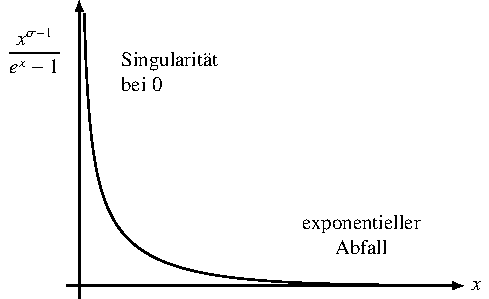
\includegraphics{papers/hankel/images/mellin-integrand.pdf}
%	\begin{tikzpicture}[scale=1.05,>=latex]
%		
%		% Achsen
%		\draw[->] (-0.2,0) -- (6.2,0)
%		node[right] {$x$};
%		
%		\draw[->] (0,-0.2) -- (0,4.6);
%		
%		% Beschriftung der y-Achse bewusst links
%		\node[anchor=east] at (-0.15,3.8)
%		{$\displaystyle\frac{x^{\sigma-1}}{e^x-1}$};
%		
%		% Kurve: nahe genug an x=0 beginnen,
%		% damit der singuläre Anstieg sichtbar wird
%		\begin{scope}
%			\clip (-0.2,-0.2) rectangle (6.2,4.6);
%			\draw[thick,domain=0.08:6,samples=200]
%			plot (\x,{(\x^0.4)/(exp(\x)-1)});
%		\end{scope}
%		
%		% Hinweise
%		\node[align=left,anchor=west] at (0.55,3.45)
%		{Singularität\\bei $0$};
%		
%		\node[align=center] at (4.55,0.82)
%		{exponentieller\\Abfall};
%		
%	\end{tikzpicture}
	\caption{Schematisches Verhalten des Mellin-Integranden für einen festen
		Realteil $1<\sigma<2$. Nur der Ursprung begrenzt das Konvergenzgebiet.}
	\label{hankel:fig:mellin-integrand}
\end{figure}
